\documentclass[11pt]{amsart}

\textwidth 6.3in

\evensidemargin=-0.1cm \oddsidemargin=-0.1cm

\textheight 8.1in

\usepackage{comment}
\usepackage{listings}
\usepackage{xcolor}
\usepackage{enumitem}
\usepackage{url}
\usepackage{graphicx}

% Configure code listings
\lstset{
    basicstyle=\ttfamily\small,
    breaklines=true,
    frame=single,
    backgroundcolor=\color{gray!10},
    keywordstyle=\color{blue}\bfseries,
    commentstyle=\color{green!60!black},
    stringstyle=\color{red},
    showstringspaces=false,
    tabsize=4
}


\begin{document}

\begin{center}
\huge HW3 \\
50pts \\

\Large Posted Friday, October 3

\Large Due Thursday, October 16

\normalsize
\end{center}

Submit written part in \texttt{HW3Solutions.pdf} and code in \texttt{predictive\_rec\_descent.py} and \texttt{predictive\_rec\_descent.pl}. Submission size limit is 2.5MB. 

\vspace{0.2in}

\noindent{\bf Problem 1} (20pts). Consider the pseudocode with nested subroutines:


\begin{verbatim}
procedure main
     g : integer
       
     procedure B(a : integer) 
          x : integer

          procedure A(x : integer)
               g := x
                  
          procedure R(m : integer)
               write_integer(x)
               x /:= 2 -- integer division 
               if x > 1
                   R(m + 2)
               else
                   A(m + 1)
              
          -- body of B
          x := a * a
          R(1)
          
     -- body of main
     B(3)
     write_integer(g)   
                      
\end{verbatim}

\begin{itemize}

\item[a)] (5pts) What does the program print under static scoping? 

\begin{verbatim}
 Output:  9
          4
          2
          6
\end{verbatim}

\newpage

\item[b)] (5pts) Show the frames on the stack when A has just been called assuming static scoping rules. Show the static and dynamic links of each frame, as well as the local variables and their values right after the assignment \texttt{g := x}. Explain how \texttt{A} finds \texttt{g}.

\vspace{0.2in}

\begin{center}
     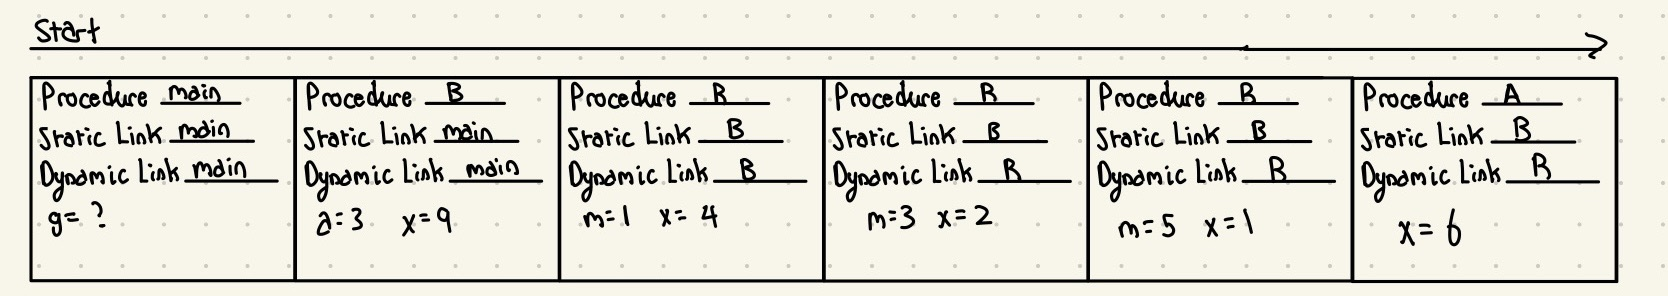
\includegraphics[width=0.9\textwidth]{IMG_0084.jpg}
\end{center}

\vspace{0.2in}


\item[c)] (5pts) Now, what does this program print under dynamic scoping?
\item[d)] (5pts) Explain how \texttt{R} finds \texttt{x} under dynamic scoping rules.

\end{itemize}


\vspace{1in}


\noindent{\bf Problem 2} (30pts). The grammar below
generates boolean expressions in prefix form:

\[\begin{array}{lll}
\mathit{start} & \rightarrow & \mathit{expr} \ \texttt{\$\$} \\
\mathit{expr} & \rightarrow & \texttt{or}\ \mathit{expr} \ \mathit{expr} \ | \ \texttt{and} \ \mathit{expr} \ \mathit{expr} \ | \ \texttt{not}\ \mathit{expr} \ | \ {\texttt {id}} \\
\end{array}\]

\begin{itemize}

\item[a)] (5pts) Write an attribute grammar (in pseudocode) to translate expressions into fully parenthesized infix form. For example, 
expression \texttt{and and a or b c d} turns into the following fully parenthesized expression \texttt{((a and (b or c)) and d)}. 
\item[b)] (5pts) Now write an attribute grammar (in pseudocode again) to translate the expressions into \emph{parenthesized} 
expressions in infix form \emph{without redundant parentheses} assuming the standard convention: unary \texttt{not} has highest precedence, 
followed by \texttt{and}, followed by \texttt{or}, and \texttt{and} and \texttt{or} are left-associative. For example, the above expression 
turns into \texttt{a and (b or c) and d}. \emph{Hint:} Assign a precedence attribute $\mathit{prec}$ to operators and expressions. 
In part c) and part d) you will code your solution respectively in Python and in Prolog. 

\item[c)] (10pts) Code in Python a predictive recursive descent parser for the grammar that also does infix translation without redundant parentheses. (Note that we can code such a parser because the grammar is LL(1).) For simplicity, assume that identifiers are lower-case letters from \texttt{a} to \texttt{z} and that the input has already been tokenized. Submit file \texttt{predictive\_rec\_descent.py} with function \texttt{parse}. \texttt{parse} takes the input list of tokens and outputs the properly parenthesized infix string if the input is in the language. It produces the empty string otherwise. Follow the structure of recursive descent from lecture (e.g., Lecture4, slides 9 and 10).  Here is how Submitty runs the function: 

\begin{lstlisting}[language=Python]
python -i predictive_rec_descent.py
>>> parse(['and','and','a','or','b','c','d'])
a and ( b or c ) and d
>>> parse(['and','and','a','or','b','c'])

>>> parse(['and','a','and','b','c'])
a and ( b and c )

\end{lstlisting}

\item[d)] (10pts) Now code the same parser in Prolog. Submit file \texttt{predictive\_rec\_descent.pl}

\begin{lstlisting}[language=Prolog]
?- parse([and,and,a,or,b,c,d],R).
R = 'a and ( b or c ) and d' ;
false.

?- parse([and,and,a,or,b,c],R).
false.

?- parse([and,a,and,b,c],R).
R = 'a and ( b and c )' ;
false.
\end{lstlisting}


\end{itemize}

\end{document}
